\documentclass[12pt]{book}

\usepackage[top=1.0in, bottom=1.0in, left=1.0in, right=1.0in]{geometry}

\usepackage{graphicx}

\usepackage{indentfirst}
\usepackage{listings}
\lstset{breaklines=true}

\usepackage{pdfpages}

\usepackage{lscape}


\author{Brian Kennedy \\ Pete Koehn \\ Theodore Lindsey}
\title{Homework 4 \\ Write up}

\begin{document}
\maketitle
\newpage

\tableofcontents
\newpage
%%%%%%%%%%%%%%%%%%%%%%%%%%%%%%%%%%%%%%


\section{Documentation}
Files needed in order to run:
\begin{itemize}
\item \_\_init\_\_.py
\item cController.py
\item cModel.py
\item cView.py
\item hw04.py
\end{itemize}

To run, place all files in the same directory, then execute the command "python hw04.py" from the command prompt or command line.

\section{hw04.py}
\hrule
\lstset{language=Python}
\lstinputlisting{hw04.py}
\hrule
\vspace{1cm}

\section{cController.py}
\hrule
\lstset{language=Python}
\lstinputlisting{cController.py}
\hrule
\vspace{1cm}

\section{cView.py}
\hrule
\lstset{language=Python}
\lstinputlisting{cView.py}
\hrule
\vspace{1cm}

\section{cModel.py}
\hrule
\lstset{language=Python}
\lstinputlisting{cModel.py}
\hrule
\vspace{1cm}


\section{Diagrams}
\begin{figure}
\caption{Sequence Diagram}
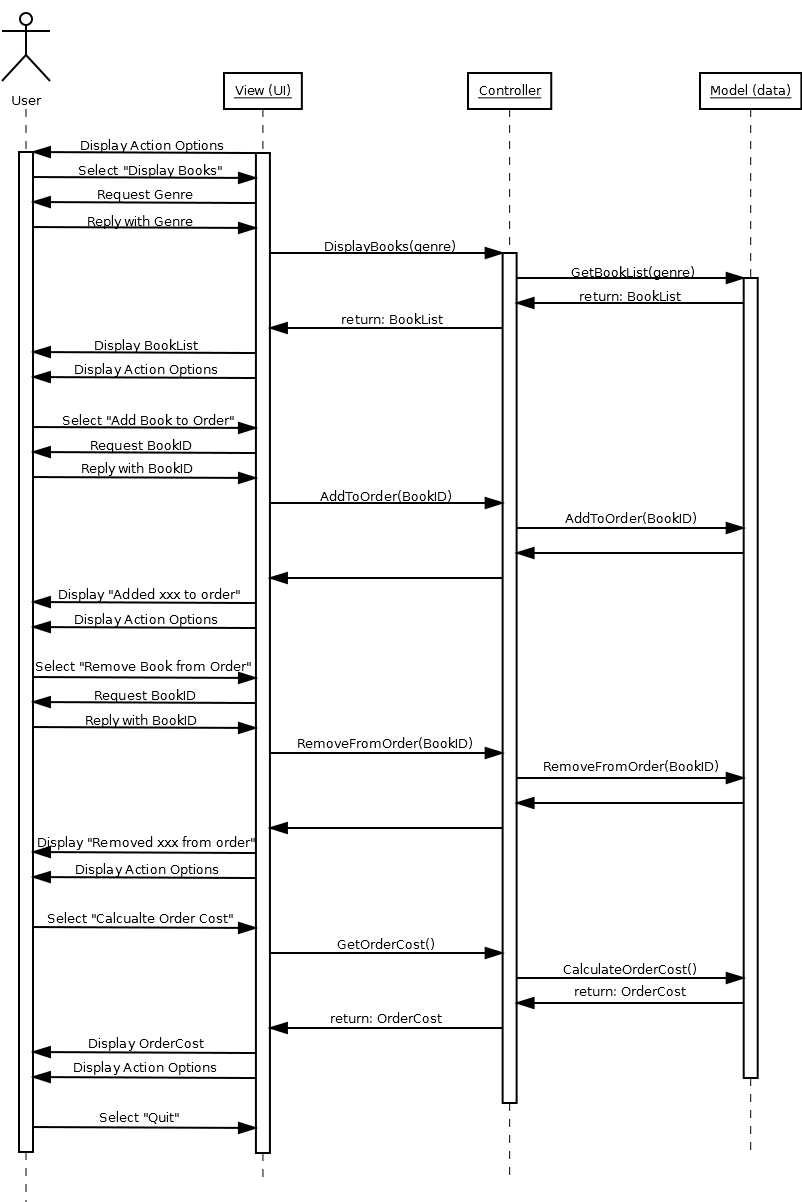
\includegraphics[height=\textheight]{dSequenceDiagram.png}
\end{figure}

\begin{landscape}
\begin{figure}
\caption{Class Diagram}
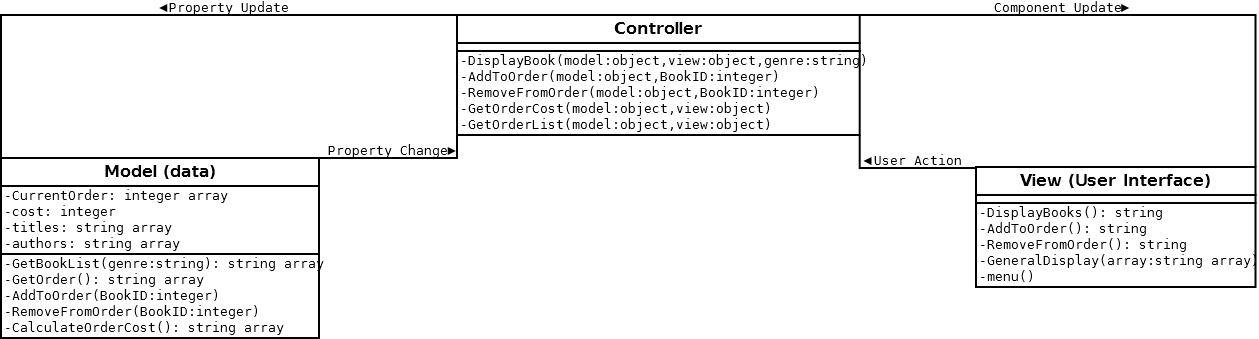
\includegraphics[width=1.3\textheight]{dClassDiagram.png}
\end{figure}
\end{landscape}


\end{document}